This section presents the results of running the system described in section \ref{ch:implementation}, with the goal of investigating performance of the EKF with real, raw data.\\ 


% Drawn path used as reference for lat lon
% px used as imperfect reference with regards to height because of extra sensors
% 
The tests were carried out taking the payload by foot along a path drawn up before testing. The path was laid along a number of small roads to make it easy to follow and thus minimize the difference between it and the actual path taken. This is therefore used as a reference for position in the horizontal plane as latitude and longitude coordinates. Additionally, position, as well as velocity, is compared with the separate PixHawk estimates. The RTKLIB position estimates are included as well.\\

\section{Stationary tests}

\section{Dynamic tests}
    \subsection{GNSS only}
    \begin{figure}
        \centering
        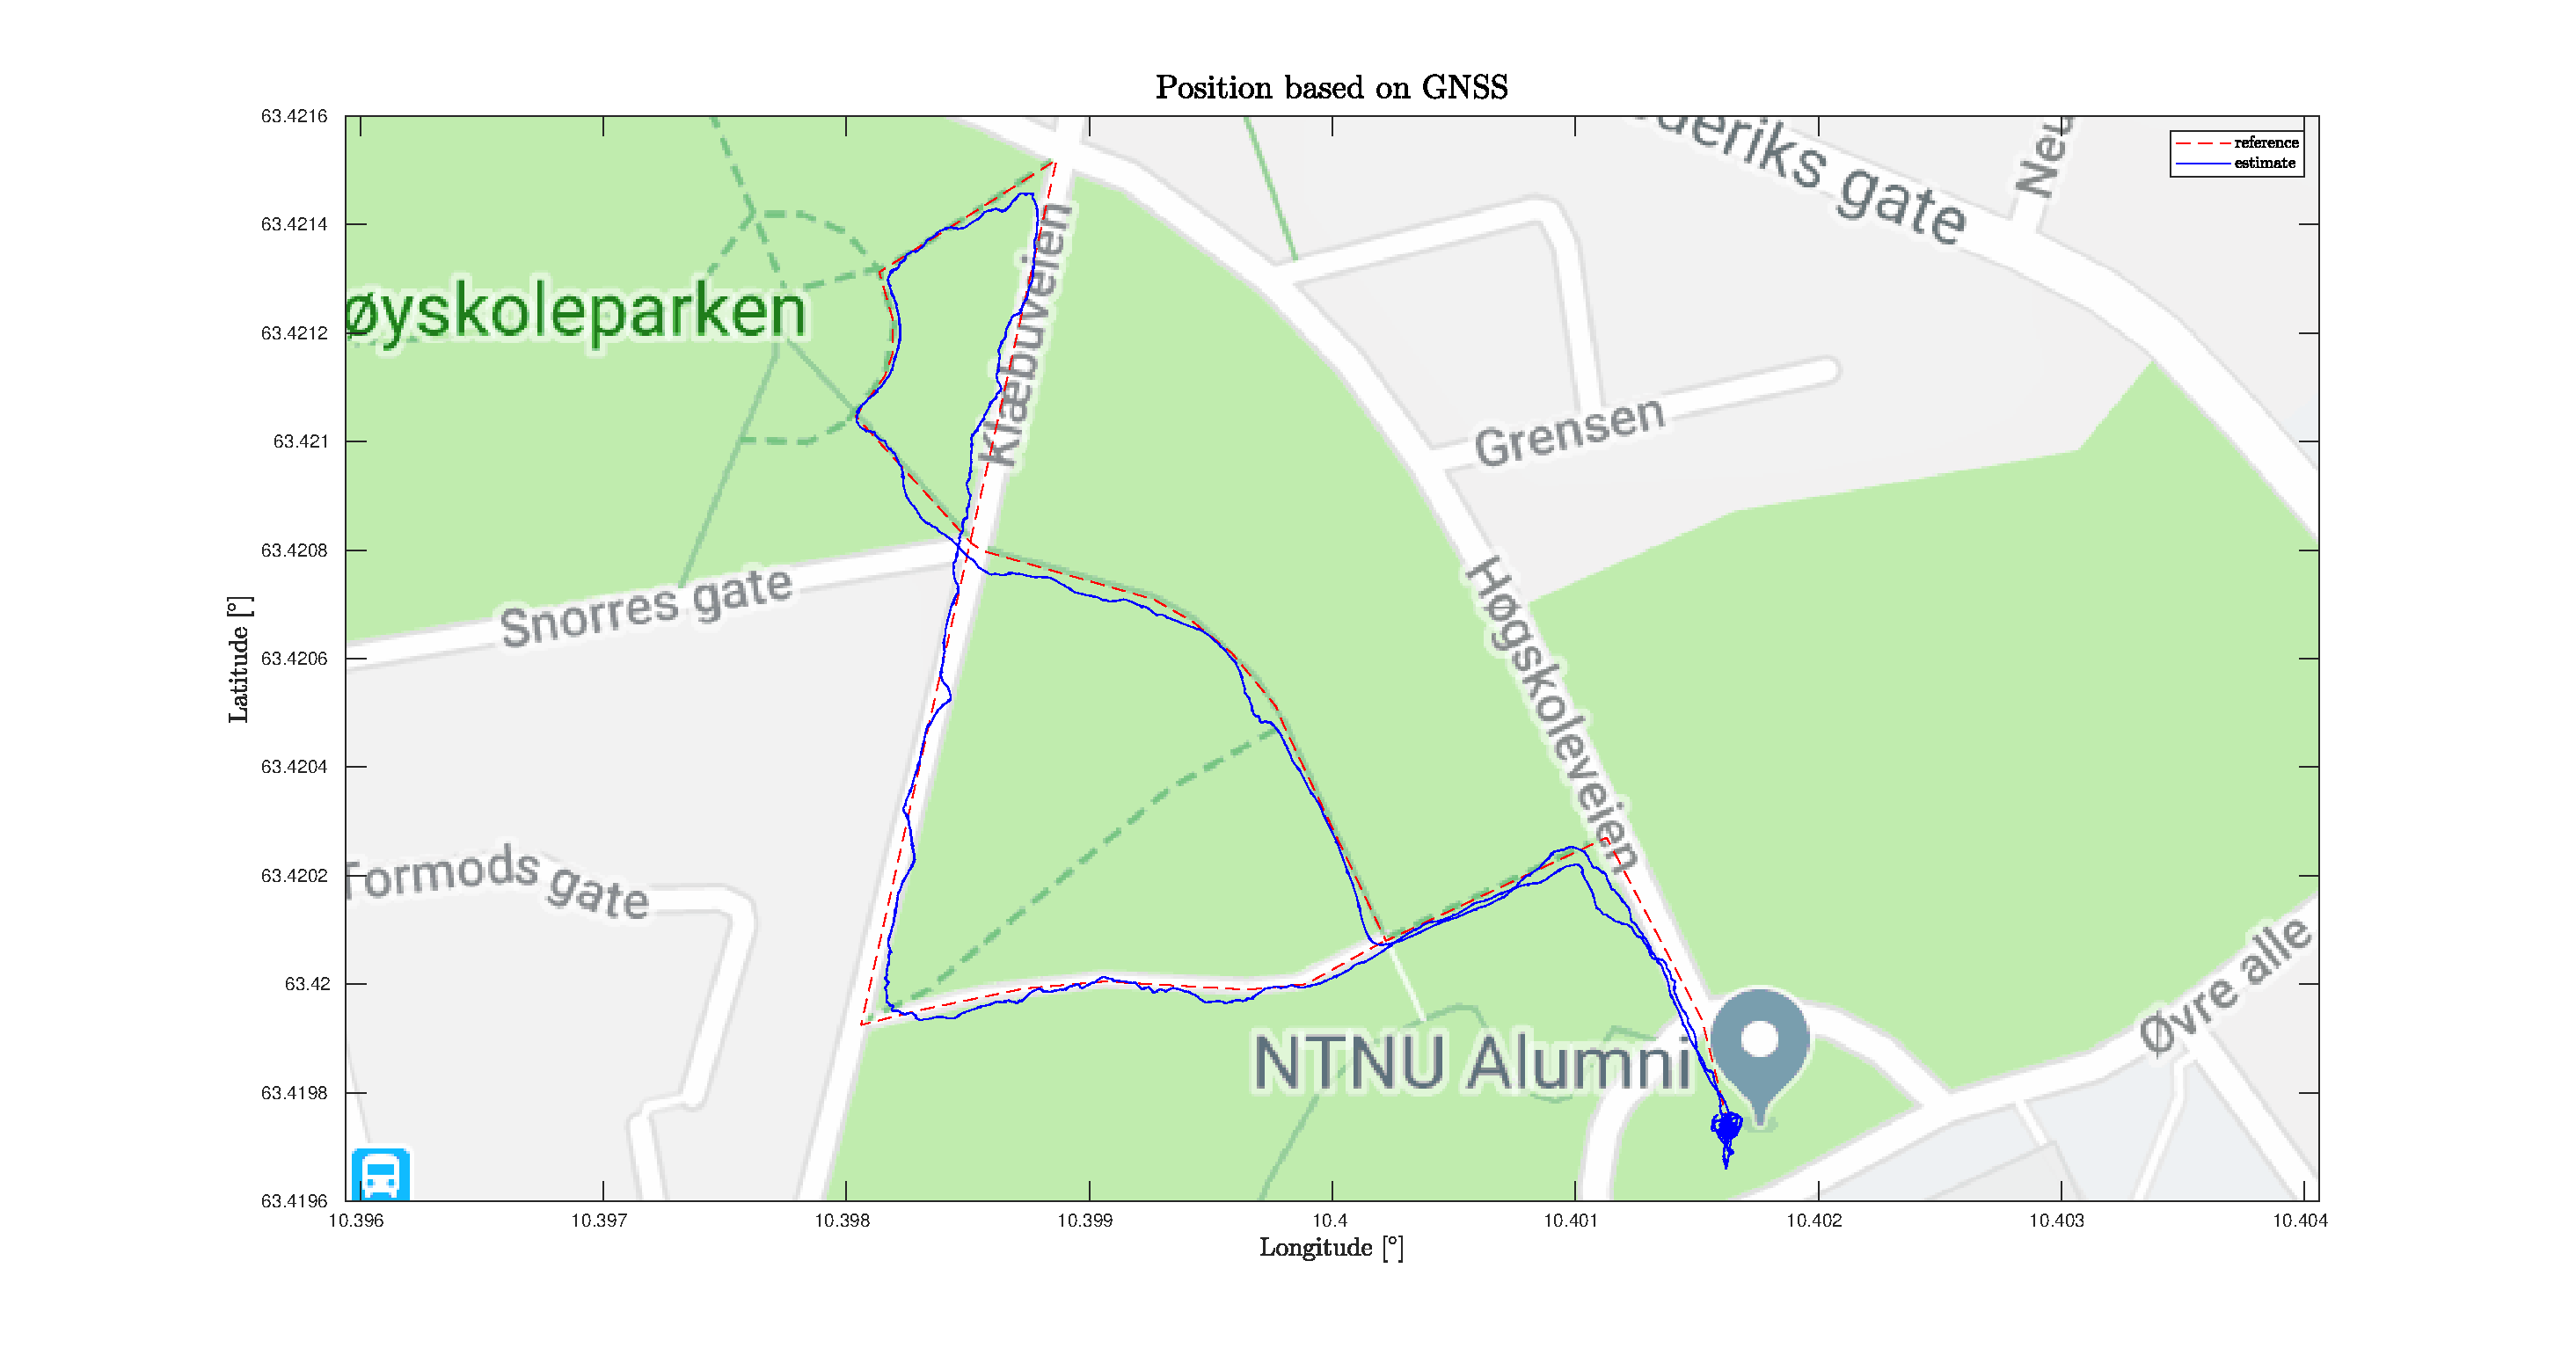
\includegraphics[scale=0.3]{Results/Images/gnss-only.eps}
        \caption{Position estimate based on GNSS measurements only}
        \label{fig:test-gnss}
    \end{figure}
    
    
    
    
    
    
    
    
    
    
    
    
    
    
    
    
    
    
    
    
    
    
    
    
    
    
    
    
    
    
    
    
    
    
    
    
    
    
%\begin{comment}
%\section{Performing the tests}
%To compare the MEKF with other systems several tests were devised, keeping in mind known %limitations of each of the systems. 
%\todo{Describe tests and thoughts behind them}

%\begin{table}[!htbp]
%\caption{List of tests}
%\label{tab:tests}
%    \begin{tabular}{|l|l||p{5cm}|}
%        \hline
%        \textbf{Tested systems} & \textbf{Test description} & \textbf{Expected result}\\
%        \hline
%        Coupled/uncoupled & Circular pattern & The MEKF should show an increase in %precision compared to the     single GNSS solution.\\
%        \hline
%        Indirect/direct filter &  Highly dynamic zigzag motion & The MEKF should follow %the quickly changing     state better than the direct filter.\\
%        \hline
%        The full system & Straight line motion/square pattern & The MEKF should generally %perform better than     the other systems\\
%        \hline
%    \end{tabular}
%\end{table}%
%
%\todo{Describe test environment}
%\missingfigure[]{Ottobil}

%Structure
    % 1 - Introduction
    %     + Test location
    %     + List of compared systems
    % 2 - Performing the tests
    %     + Description of how the tests were performed (waited for steady state..)
    % 3 - Actual results
    %     + Graphs, tables, rms
    %     + 
    
\todo{Log cpu usage}

%\end{comment}

%This chapter presents the experimental results from running the system described in chapter \ref{ch:implementation}. A base station with a setup similar to the described system was set up, and the results are compared to the RTK solution of RTKLIB, as well as the internal PixHawk state estimate.